\chapter{实验验证与结果分析}

本章根据之前的模型设计,结合仿真平台对所提出的基于海量交通数据的出租车移动模型进行了编码实现,并利用仿真平台对协议的性能进行了模拟验证,对比其与实际轨迹在接触和节点分布上的相似性,并与其他传统移动模型相比较。

%出租车移动模型的实现
\section{出租车移动模型的仿真实现}
<补充在ONE平台上的扩展部分>

为了验证模型的有效性,我们在仿真平台ONE(Oppor- tunistic Networking Environment)\cite{KeranenOtt-155}上扩展实现了出租车移动模型T-START. 本节将详细介绍出租车移动模型的实现方法和相关配置。
<给出结构图>

<给出仿真结果>

\begin{figure}[ht]
\centering
\subfigure[Real Trace]{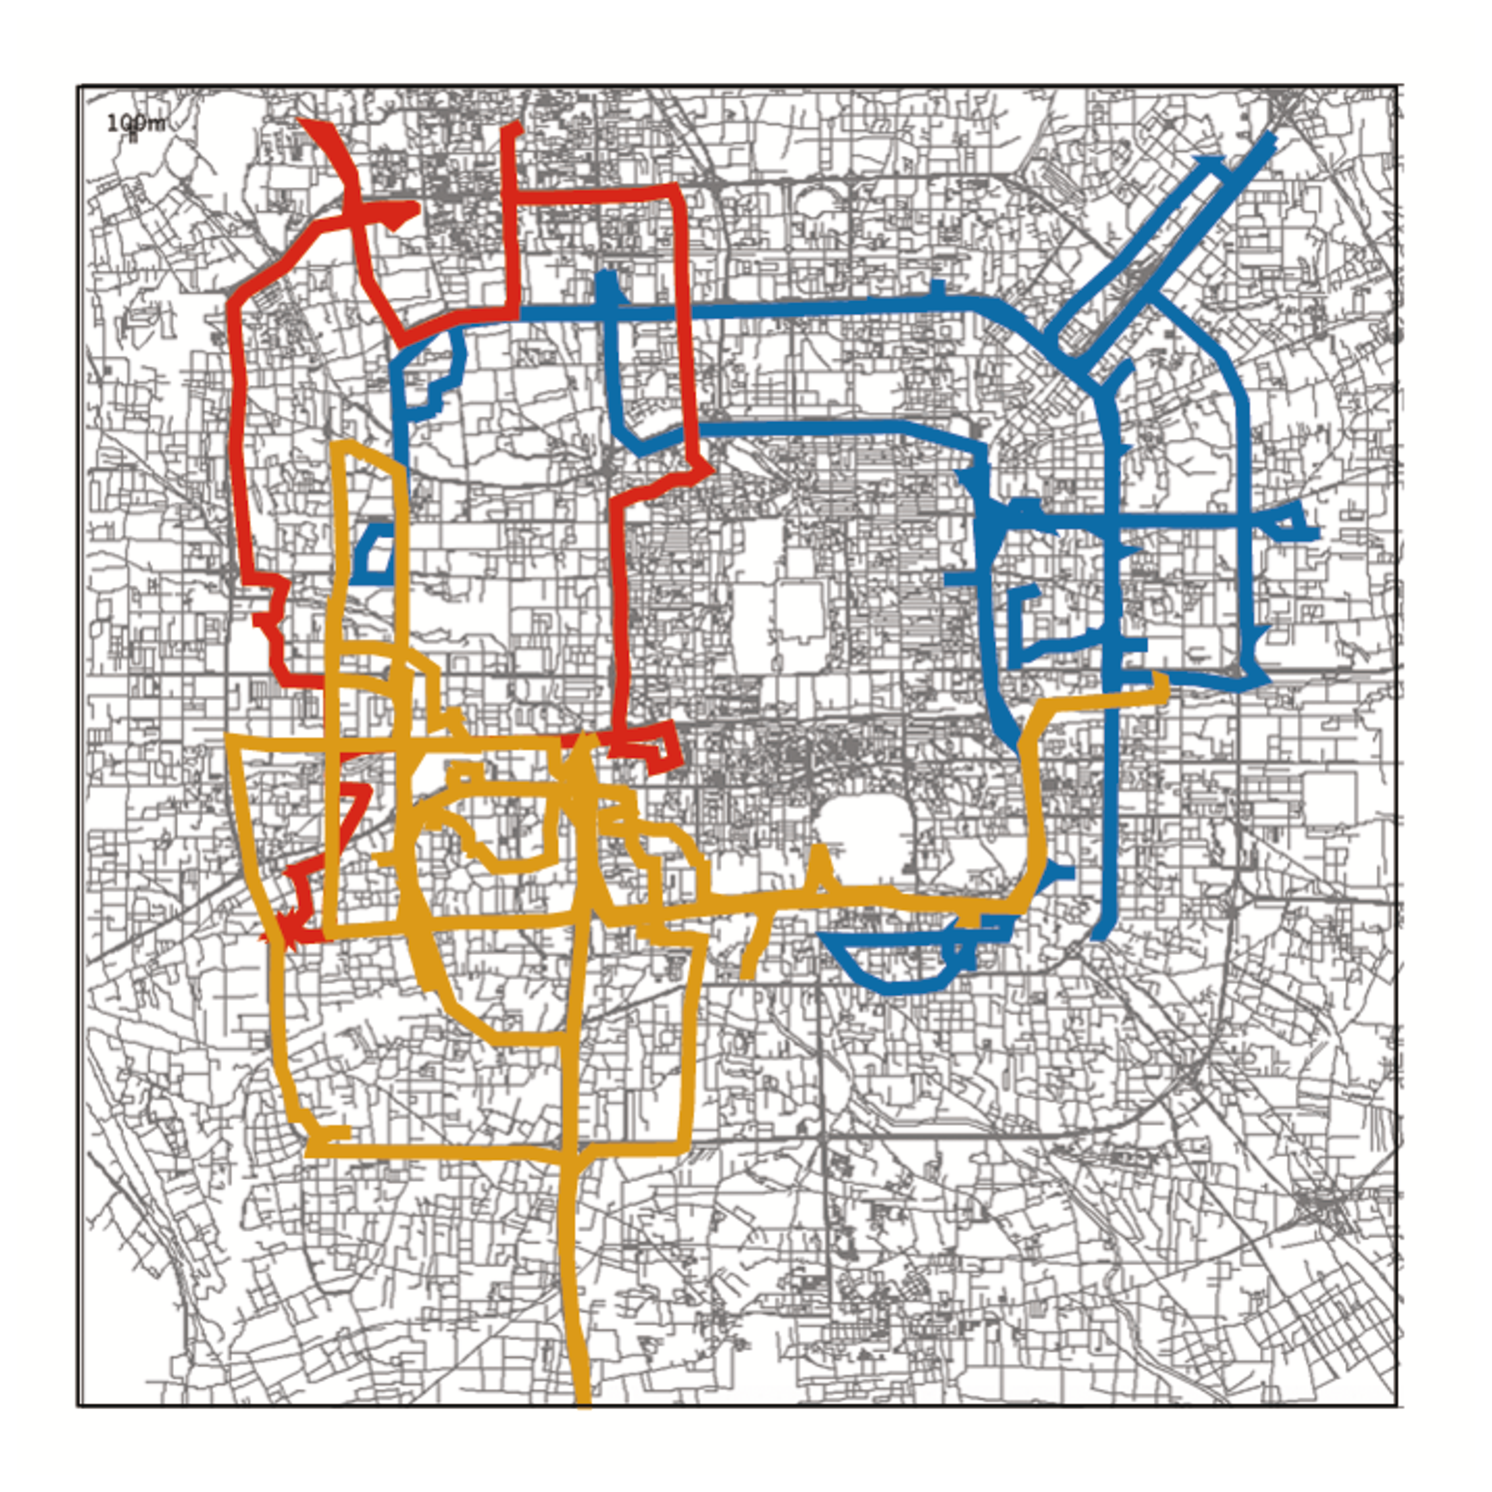
\includegraphics[width=0.24\textwidth]{figures/evalue/sample/real_traces.eps}}
\subfigure[T-START]{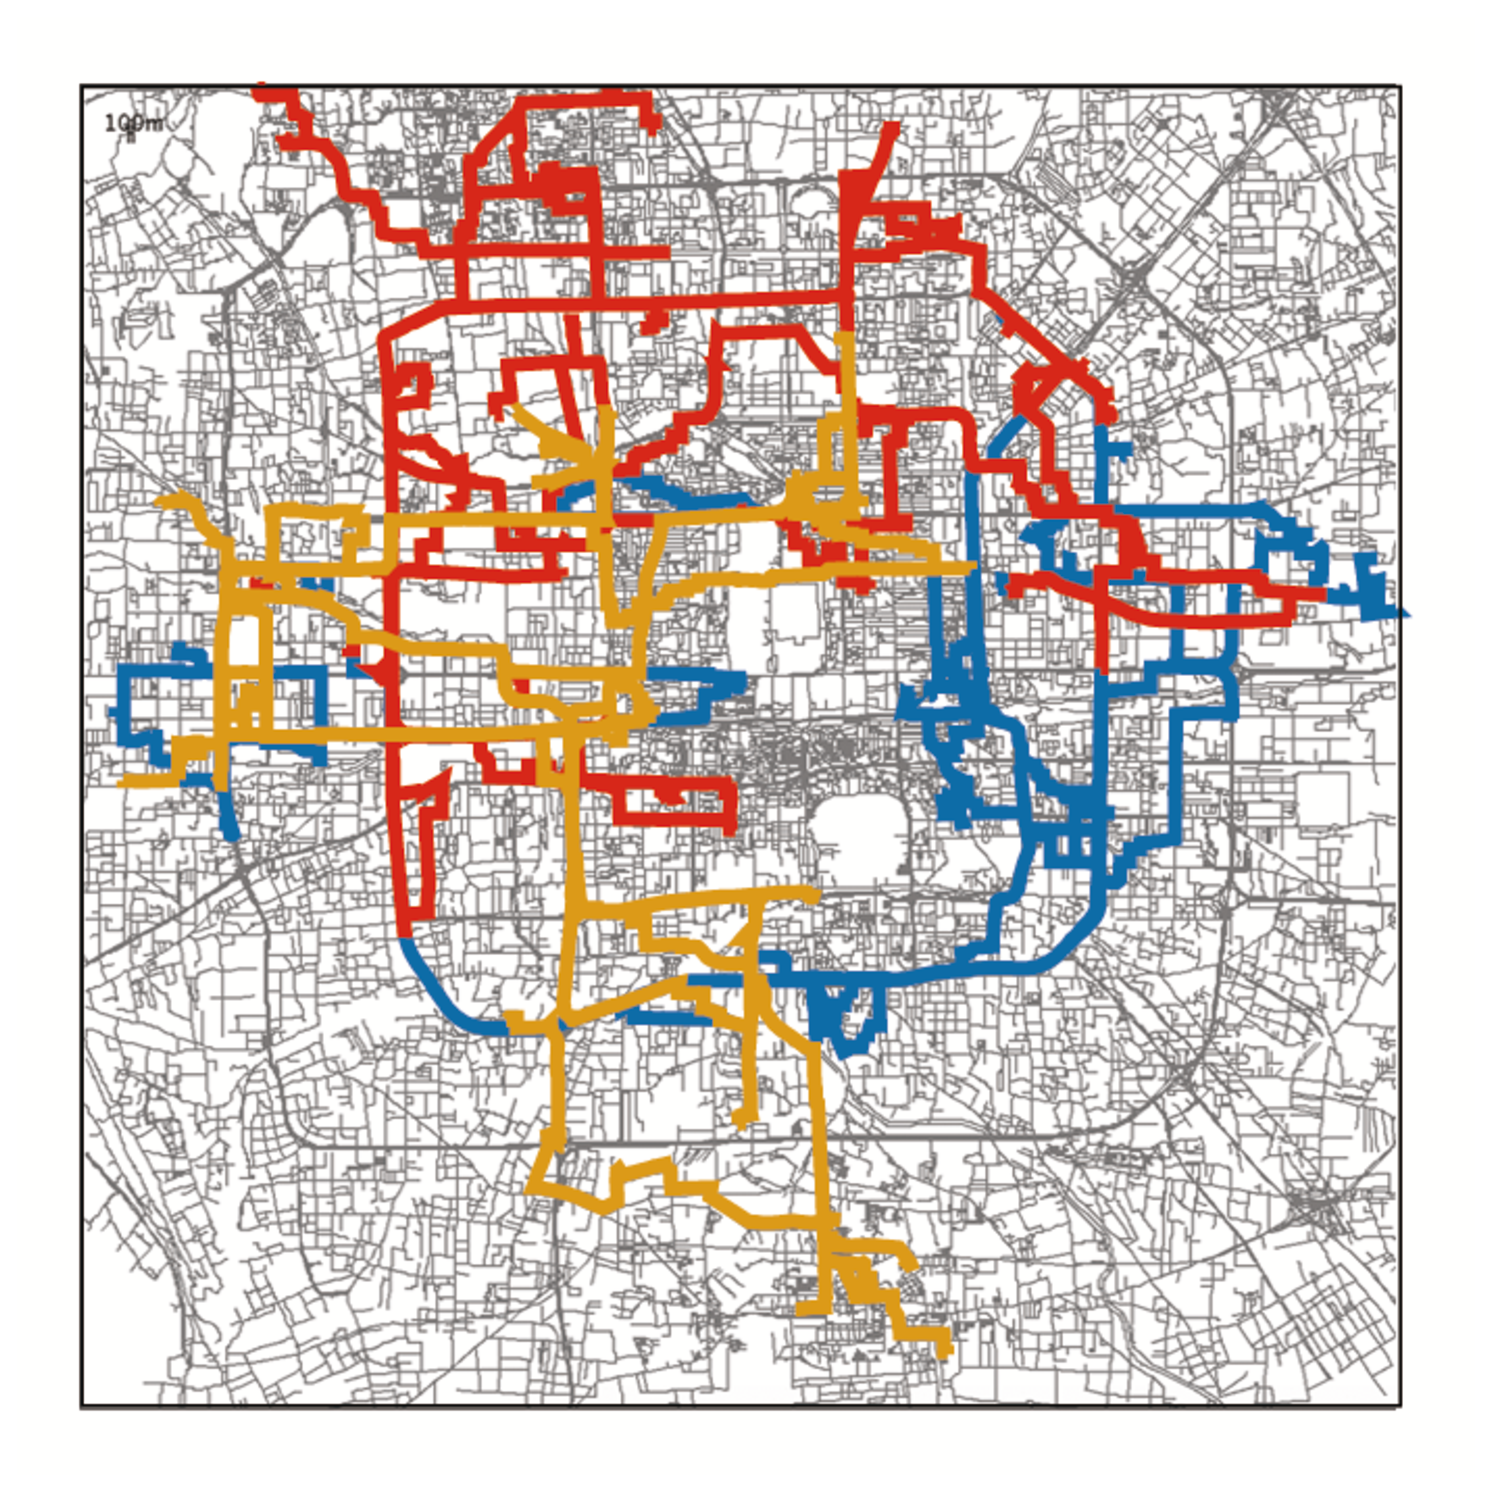
\includegraphics[width=0.24\textwidth]{figures/evalue/sample/start_traces.eps}}
\subfigure[SP]{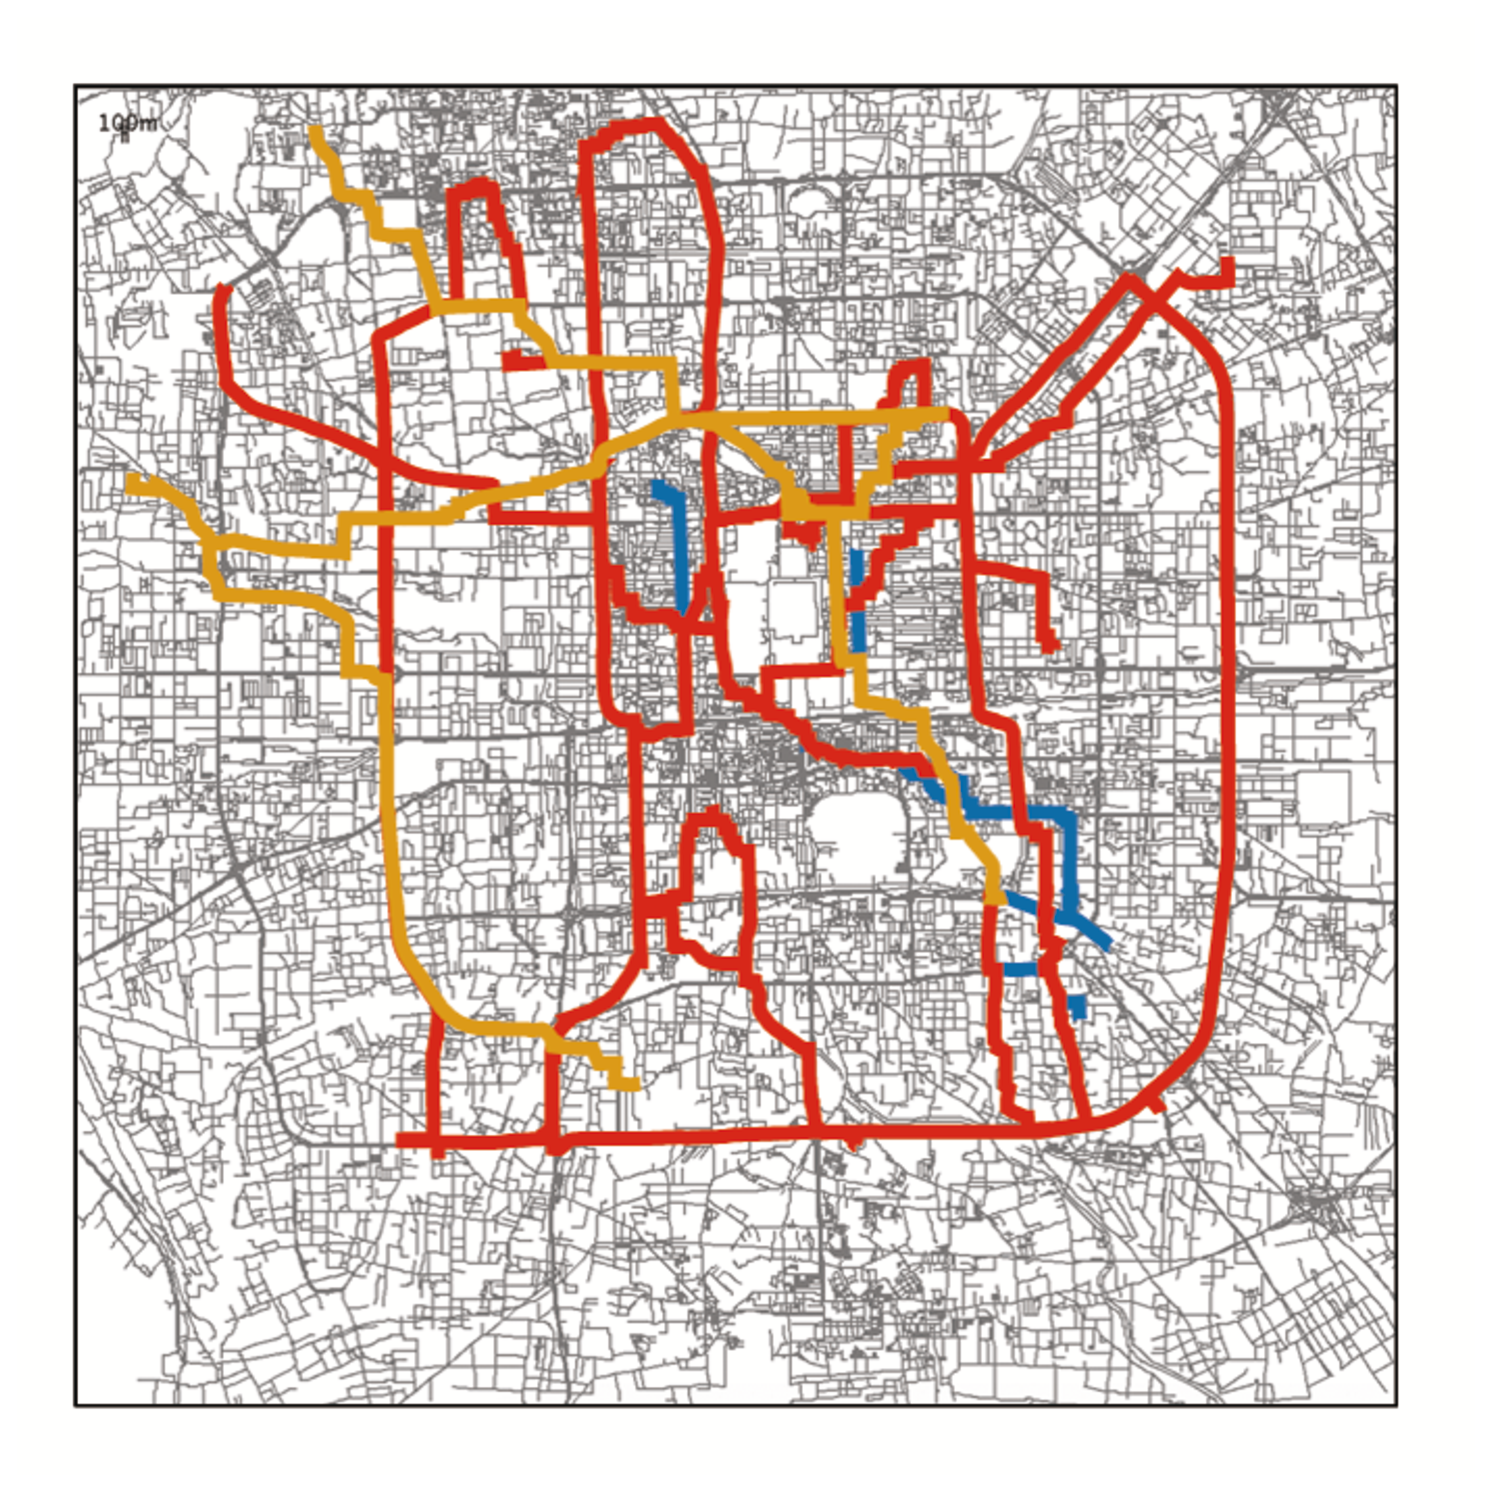
\includegraphics[width=0.24\textwidth]{figures/evalue/sample/sp_traces.eps}}
\subfigure[RWP]{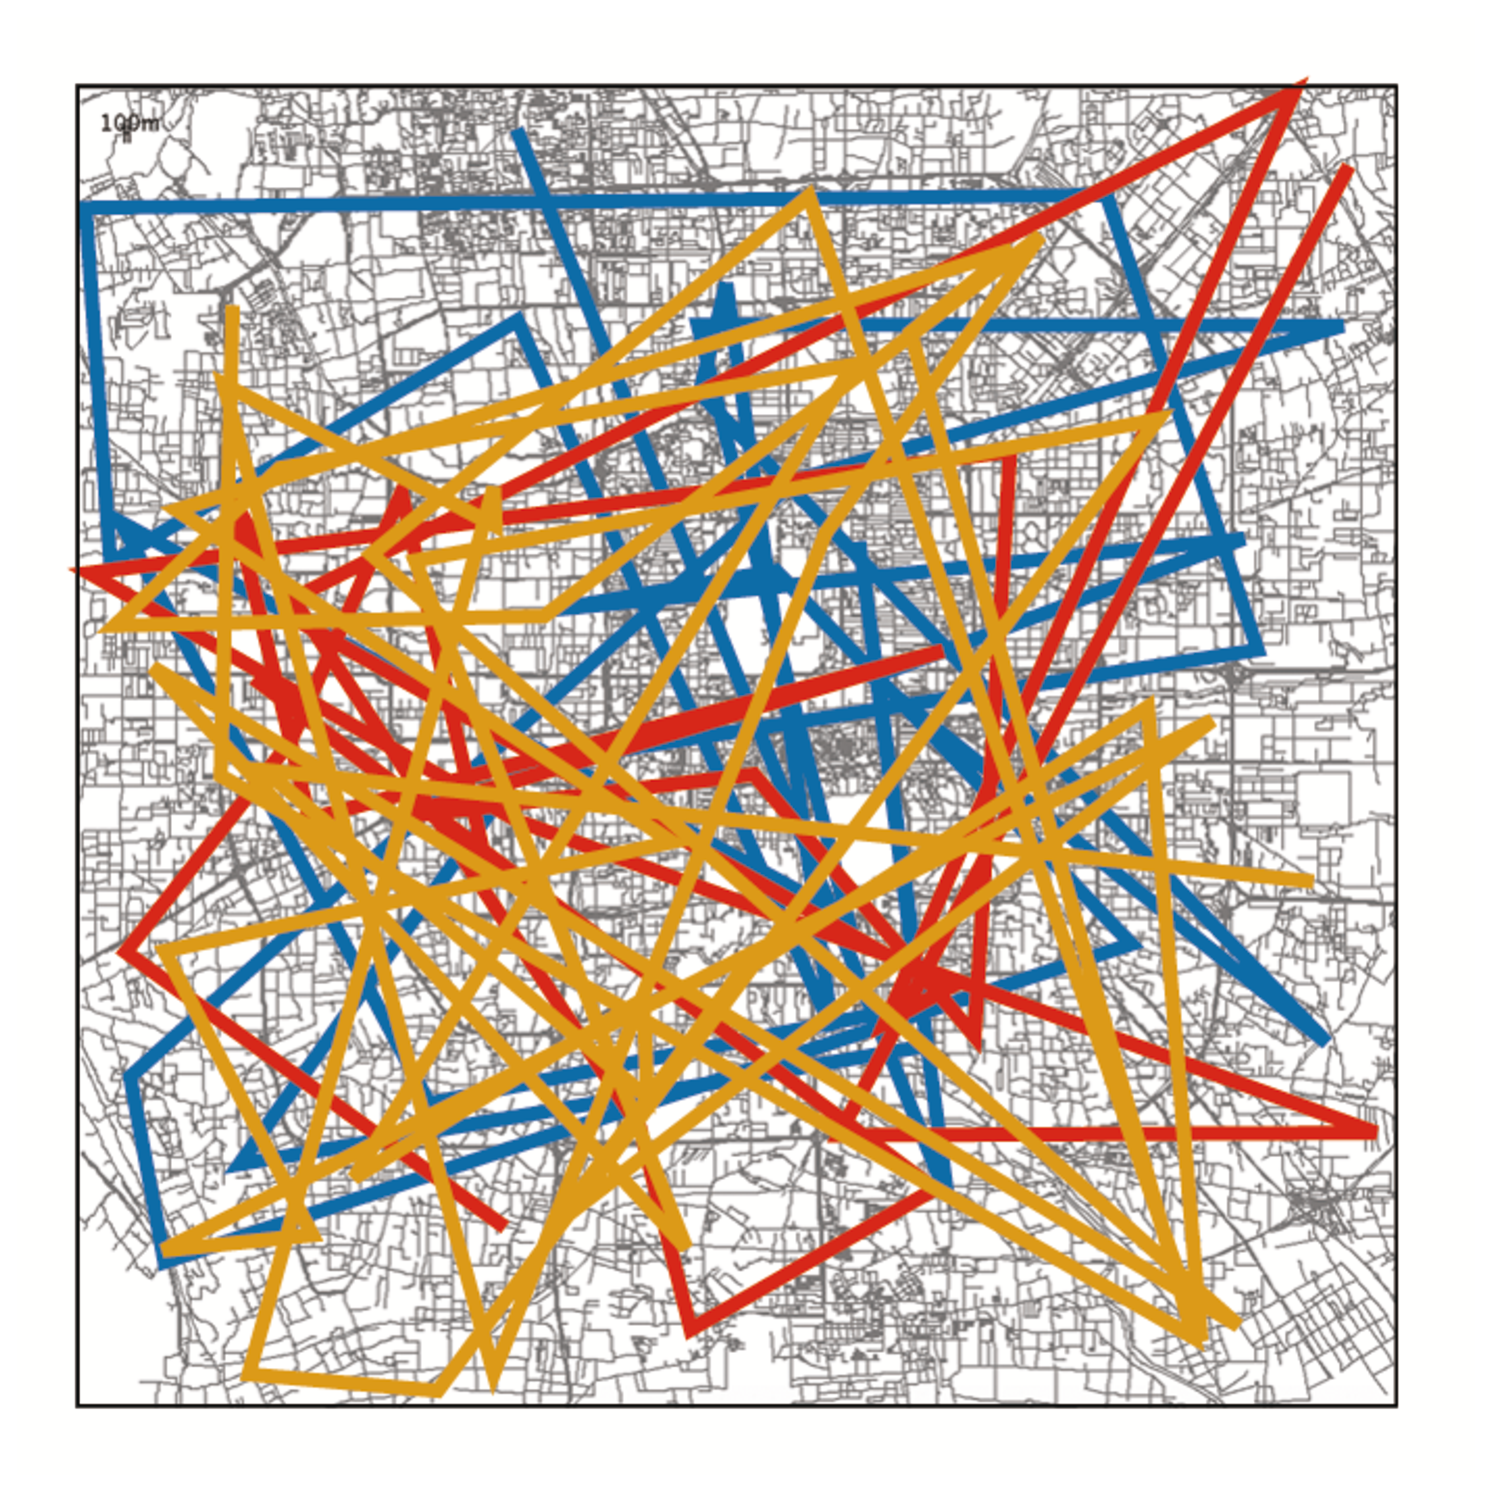
\includegraphics[width=0.24\textwidth]{figures/evalue/sample/rwp_traces.eps}}
\caption{模型生成的轨迹样例}\label{figure_tracesample}
\end{figure}

\begin{figure}[h]
\centering
\subfigure[Real Trace]{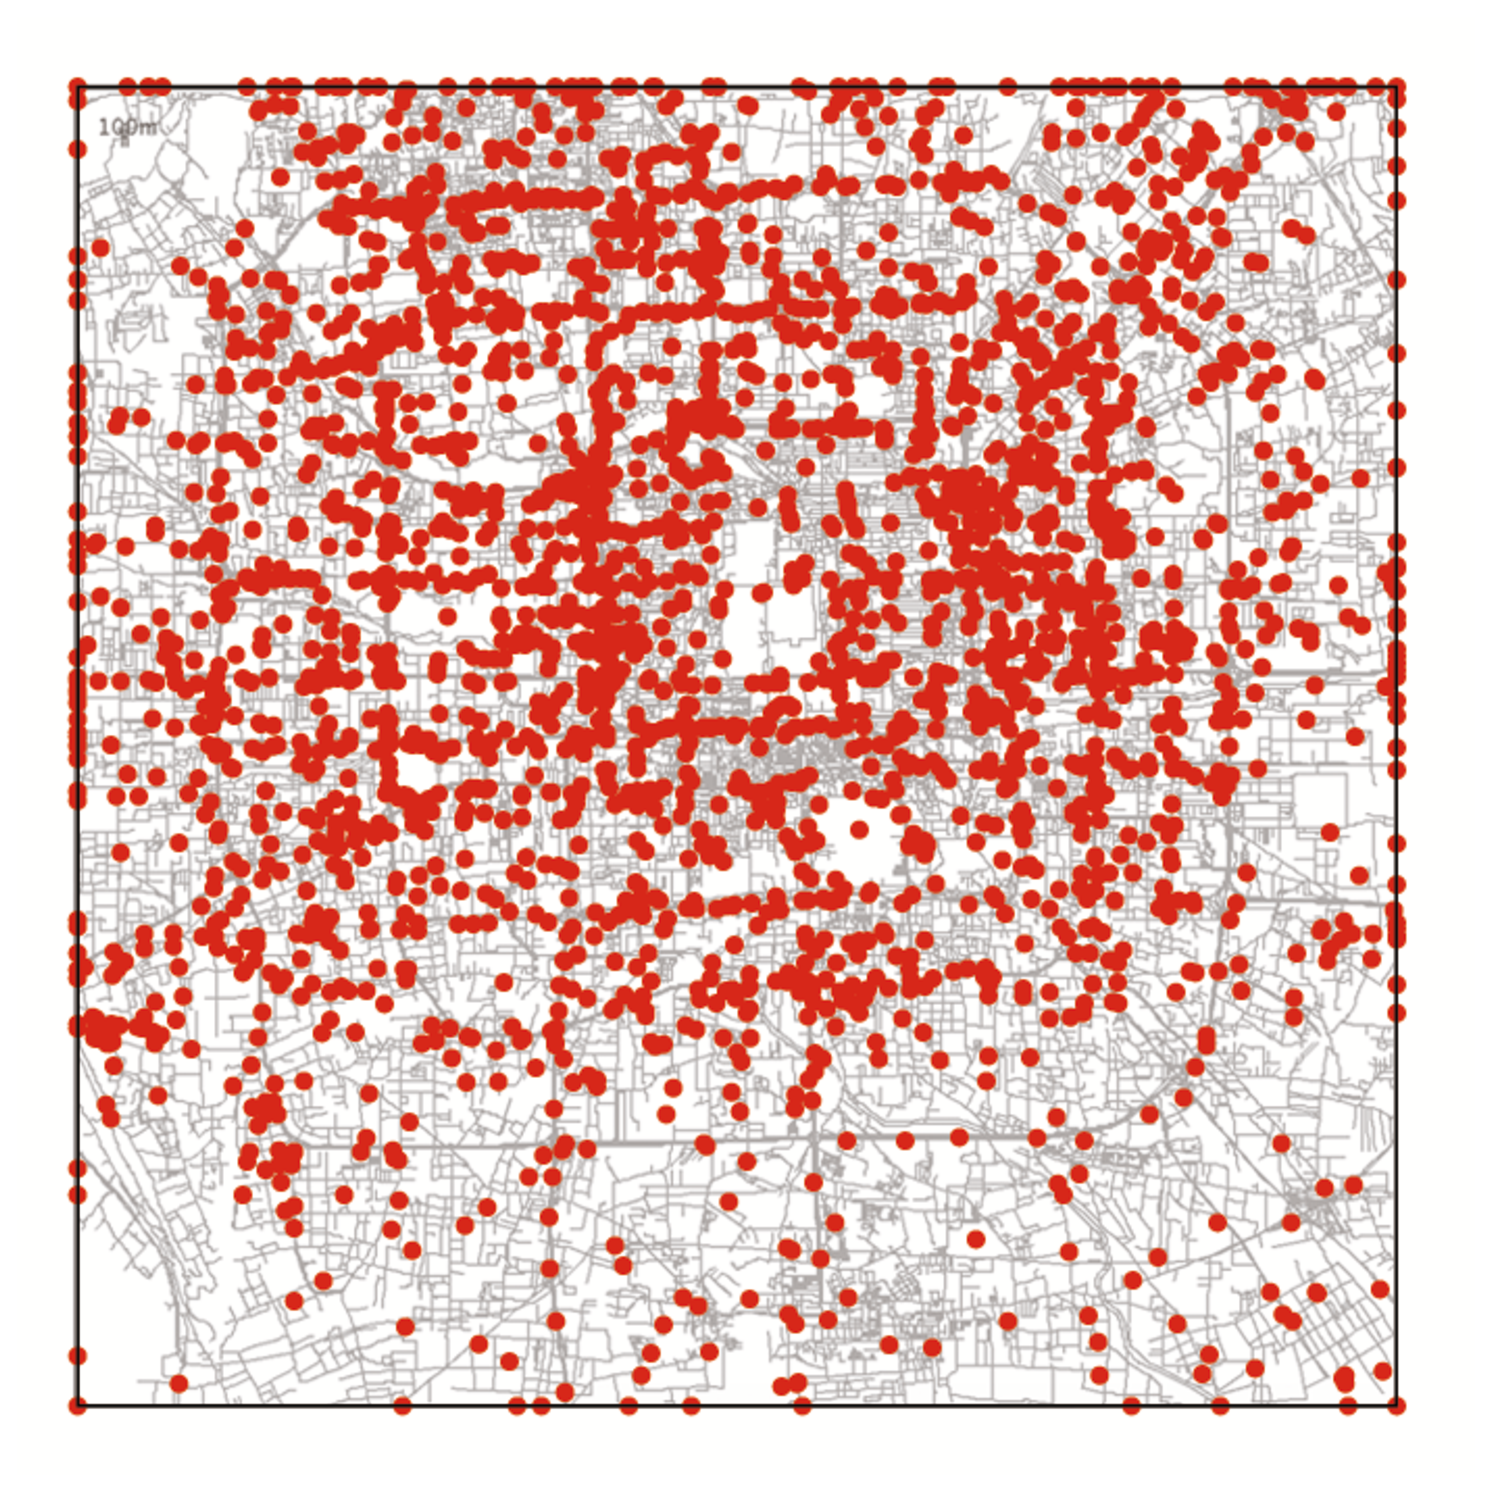
\includegraphics[width=0.24\textwidth]{figures/evalue/trace_nodedis.eps}}
\subfigure[T-START]{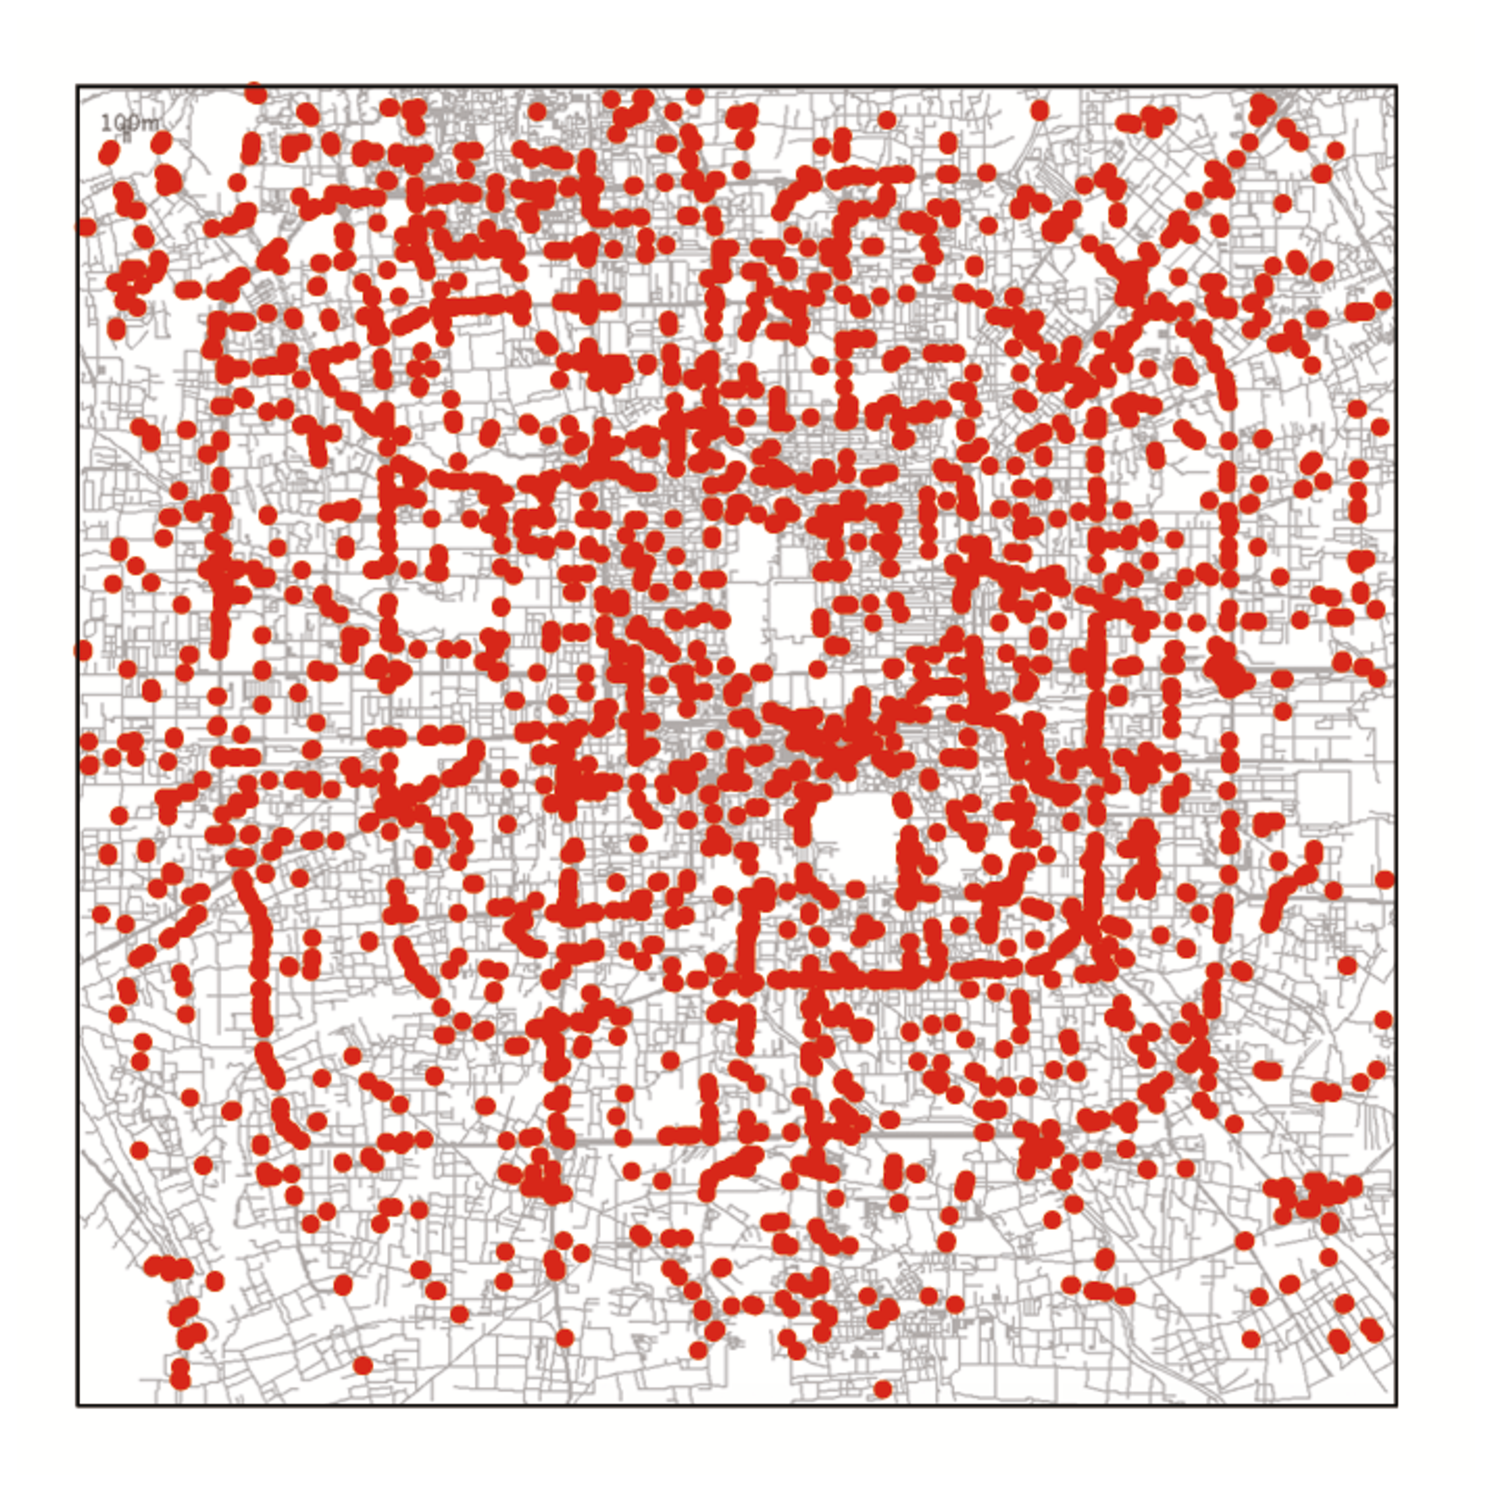
\includegraphics[width=0.24\textwidth]{figures/evalue/start_nodedis.eps}}
\subfigure[SP]{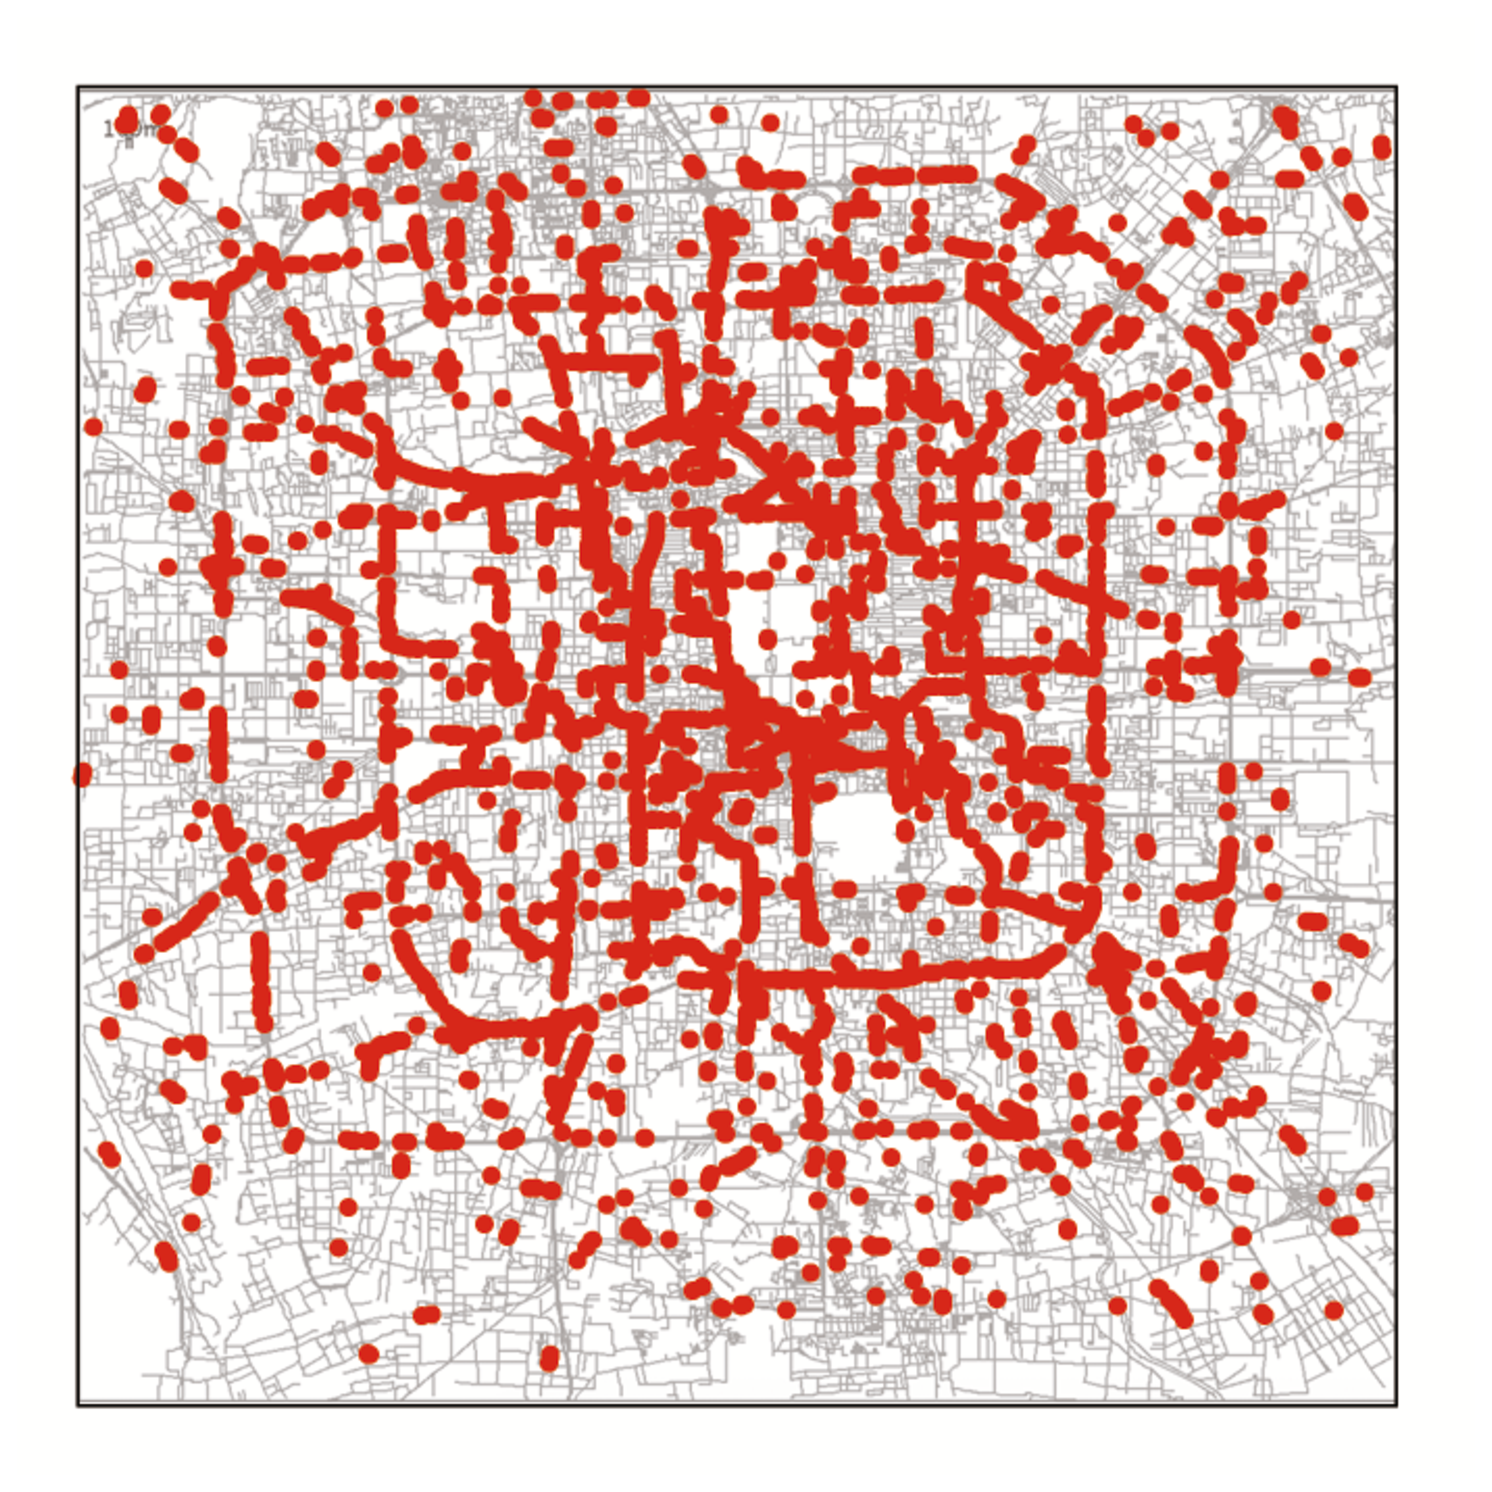
\includegraphics[width=0.24\textwidth]{figures/evalue/sp_nodedis.eps}}
\subfigure[RWP]{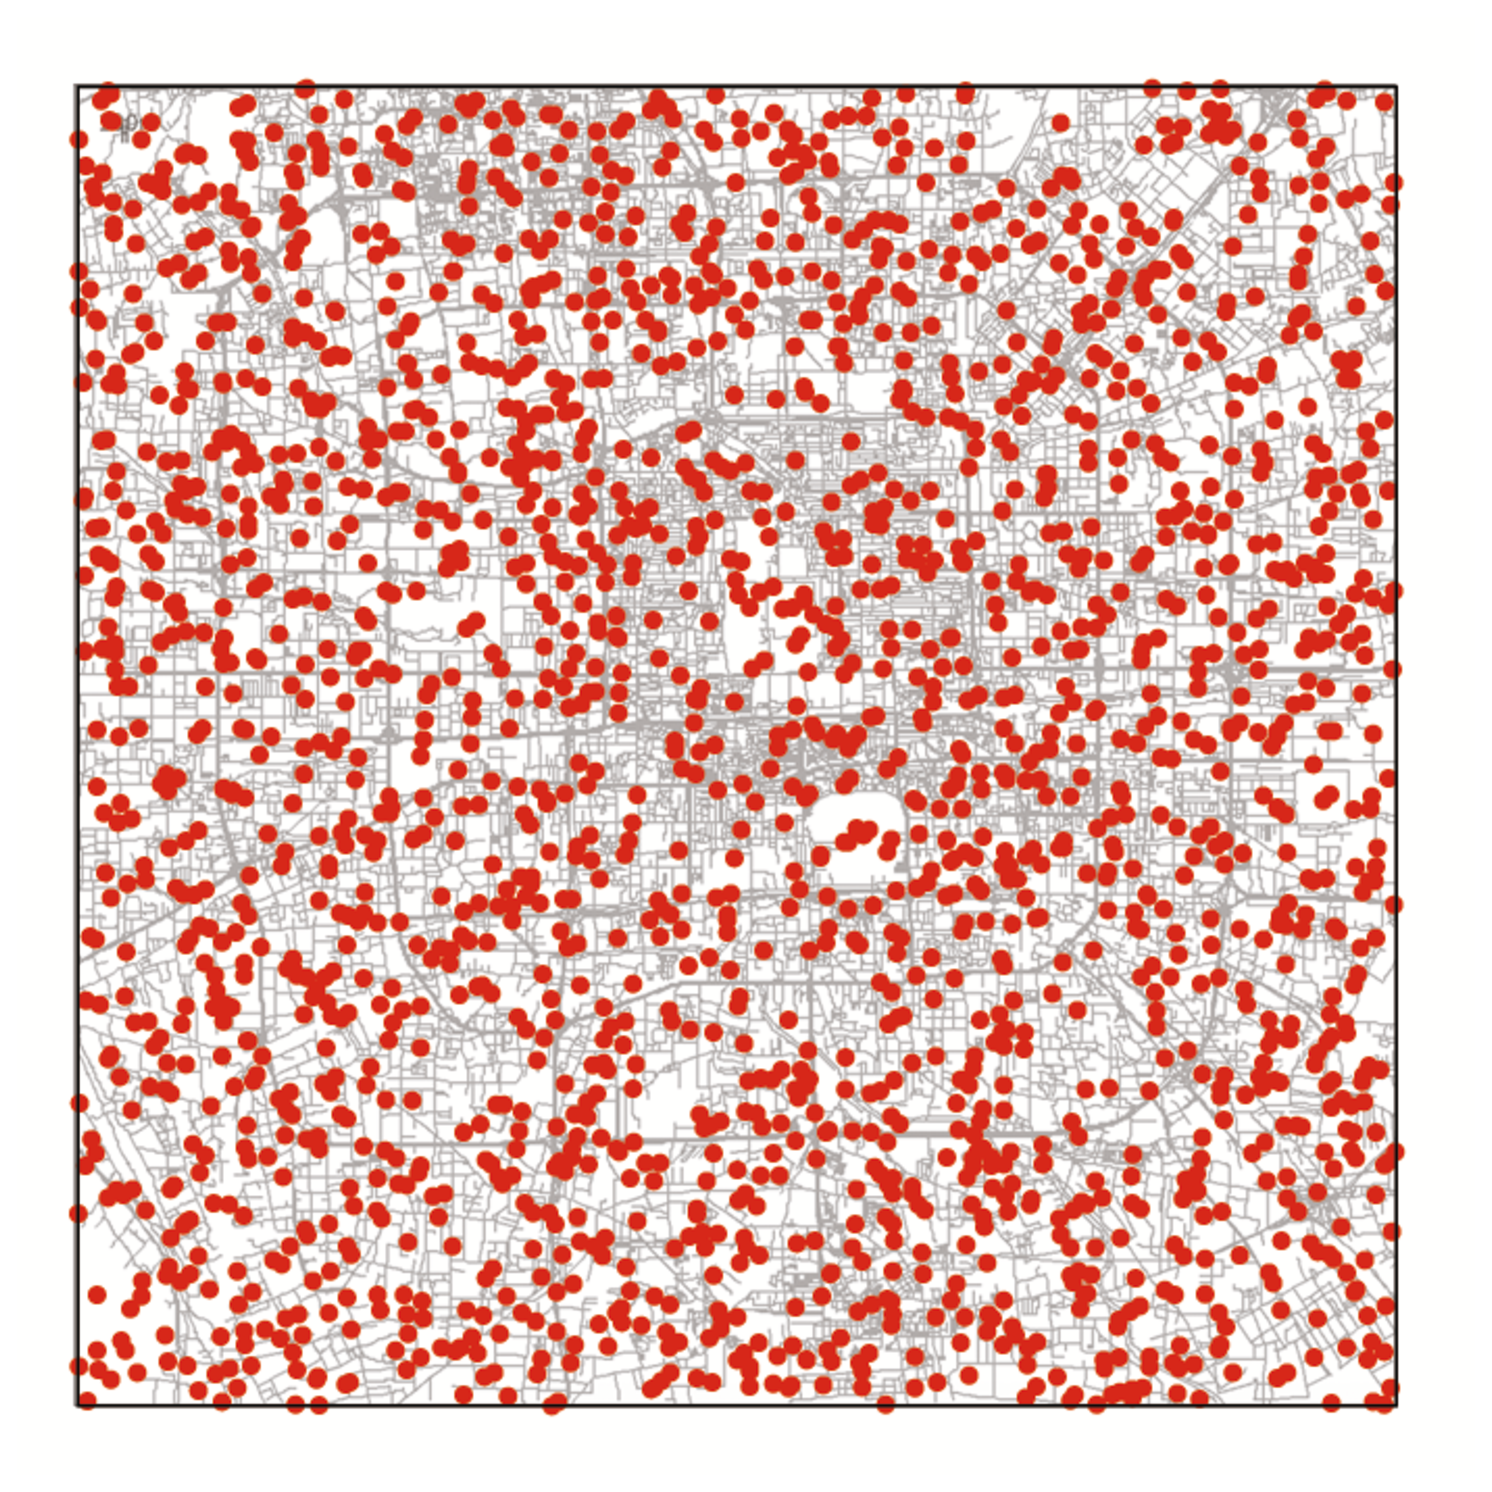
\includegraphics[width=0.24\textwidth]{figures/evalue/rwp_nodedis.eps}}
\caption{模型节点分布快照}\label{figure_trace_snapshots}
\end{figure}

Trace samples and their node distribution snapshots from different mobility models are reported in Fig.~\ref{figure_tracesample} and Fig~\ref{figure_trace_snapshots}. Fig.~\ref{figure_tracesample} shows the trace in one day. The traces of the real data and T-START only cover some parts of the area, while the traces of SP and RWP almost go through the whole area. Recall that SP and RWP select a destination randomly in the area, while T-START takes the associations between current region and destinations into consideration (which satisfies the movement rules of taxis). In Fig.~\ref{figure_trace_snapshots}, real trace, T-START and SP exhibit the road structures, while the node distribution of RWP is much uniform. As to T-START, the destination section process decides that it tends to select a destination in the regions with higher load/drop event probability. Therefore, with the decline of the randomness, the snapshot of T-START becomes much clear and centralized on the main roads, which matches real traces very well.


\section{实验配置和验证指标}

为了验证模型的有效性和准确性,我们选择了两个其他的移动模型作为比较,一个自由移动模型——随机路点模型(Random Waypoint,RWP)和一个地理限制模型——最短路径(Shortest Path, SP)移动模型。RWP是一种经典的移动模型,被广泛应用于车联网,ad hoc等环境的仿真中。SP是一种基于地图的最短路径移动模型,它基于可以配置连通的地图文件,然后每次通过随机选取目的点,然后用最短路径(Dijkstra)算法在当前点和目的点之间寻找一个最短路径并在此路径上移动。

为了验证模型的有效性,我们选取了两个角度的指标。一是节点的分布特性,一段时间点节点的分布具有实时性,其与时间的强相关性是的直接的节点分布不容易比较。因此我们引入了出入度的概念。

出入度是相对某一块区域来说的,在一段时间内进入此块区域的节点数为此块区域在这段时间内的入度。类似的,在一段时间内移动出某块区域的节点数为此块区域的出度。文献[XXX]也是用此种方式来验证移动模型的有效性的。

接触是在用于移动容迟网络,ad hoc等网络中的一个概念,可定义为一次通信的机会。在车联网通信,路由算法的研究等方面,有很多接触相关的研究[XXX]。我们选取接触作为另一个指标,来验证移动模型中节点间的关系是否在统计规律上与实际接触符合。我们定义两个车辆节点间距离小于等于一段距离时,两节点发生了接触。

仿真区域是北京市包括中心区域的$24,000\times 24,000m^2$,我
由于本文提出的移动模型考虑到了时间和空间维度,因此在实验验证时选取了四个不同时间段,分别是早上6点(6:00)到8点(8:00), 中午的11点到13点,下午的17点到19点,晚上的22点到24点。

在速度方面,T-START采用了对应时间段的车辆拟合结果,如表\ref{XXX}所示,而RWP和SP移动模型的速度为一段速度区间内的一个均匀分布产生,我们需要对之设定速度的上下限。因此我们选取了实际轨迹速度的均值的两倍作为其上限,四个时间段对应的SP和RWP的速度区间如表\ref{XXX}所示。
\begin{table}
\centering
\caption{RWP和SP的速度区间设定}
\begin{tabular}{cc}
\hline
\hline
  时间段& 速度区间 \\
  \hline
6:00-8:00  & $[0, 36.86]km/h$ \\
11:00-13:00  &  $[0, 36.86]km/h$\\
17:00-19:00 &  $[0, 30.50]km/h$\\
22:00-24:00  & $[0, 40.802]km/h$\\
\hline
\end{tabular}
\end{table}
我们随机选取了3000辆出租车作为对比对象。

%介绍RWP和SP
\section{节点分布验证}

节点分布对交通和网络性能仿真有十分重要的影响,很好的理解其节点分布规律能帮助到巡经和拥塞控制。然而节点的动态性导致了节点分布的动态性,为了量化节点分布的变化,我们引入了出入度的概念。出入度指出了在一段时间内有多少出租车驶入或驶出区域。我们将整个仿真区域划分为$400m \times 400m$的网格来探究每个网格中的出入度。时间区间为两小时,即其仿真时间为2小时。实际轨迹数据为2011年11月8日的轨迹数据。

平均的出入度结果相同,因为当一个节点离开一个区域后必然会进入另一个区域,也就是区域$i$的入度减去1,出度加1,对应的有区域$j$的入度加1,出度减$1$. 平均的出入度值如表\ref{table_avg_inoutdegree},出入度的方差如表\ref{table_variance}.

由于车辆速度的增加,中午时的车辆出入度明显出现了一个高峰。而下午5:00-7:00,可能由于车辆拥塞比较严重,使得车速放缓,因此在此时间段,平均出入度有所回落。晚间由于车辆减少,出租车行驶速度增加。图中可见,由于RWP的方向随机特性,其出入度均明显低于其他,T-START在6点到8点和17点到19点间与实际较为相符,在中午11点到13点和晚上22点到24点,T-START的均值要高于实际轨迹。而SP具有和实际轨迹较好的相似性。因此可以证明其速度的设定较为合理。

对于方差方面,SP与实际也有较好的符合性,节点的在不均匀分布方面和实际轨迹较为接近。而T-START在早上和下午的出入度的方差要低于实际轨迹。RWP的方差基本持平,符合RWP的均匀分布的特性。

以上均值和方差可以看出对于SP的速度等参数的设定较为合理,但是不能证明两者出入度的相似性,为了说明相似性,我们使用了相对误差,比较每个对应网格的值。


\begin{figure}[!h]
\centering
\subfigure[average]{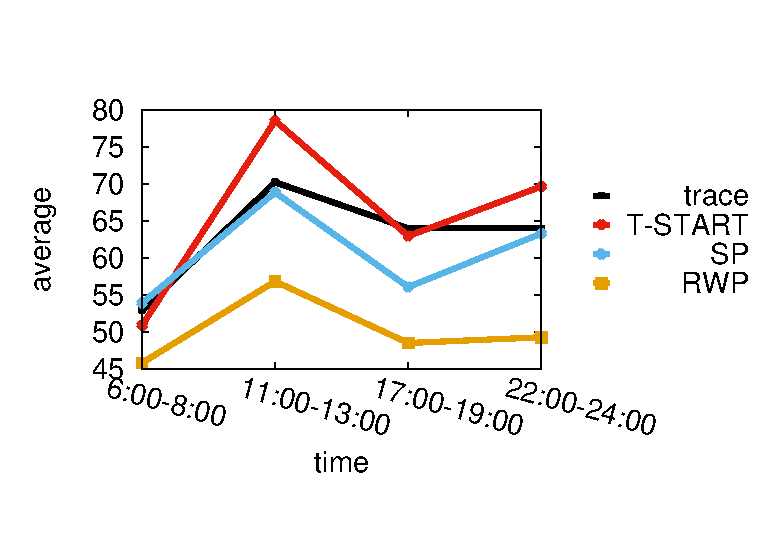
\includegraphics[width=0.5\textwidth]{figures/evalue/indegree/avg.eps}}
\subfigure[variance of in-degree]{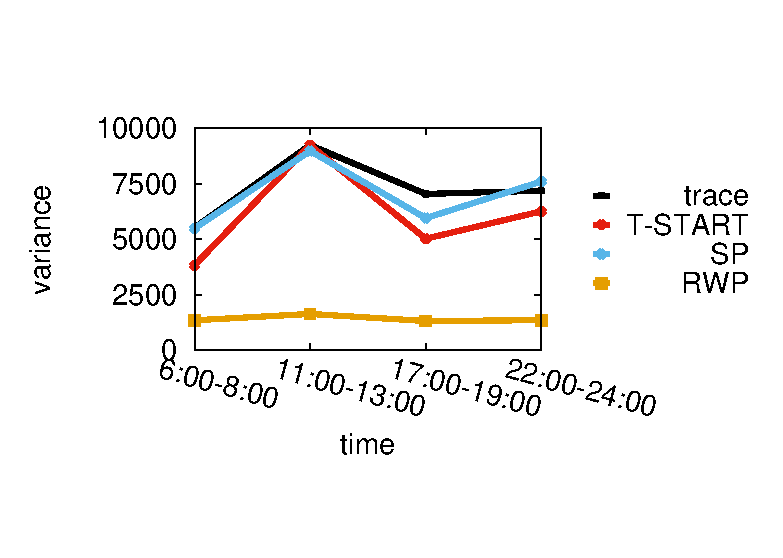
\includegraphics[width=0.5\textwidth]{figures/evalue/indegree/var_in.eps}}
\subfigure[variance of out-degree]{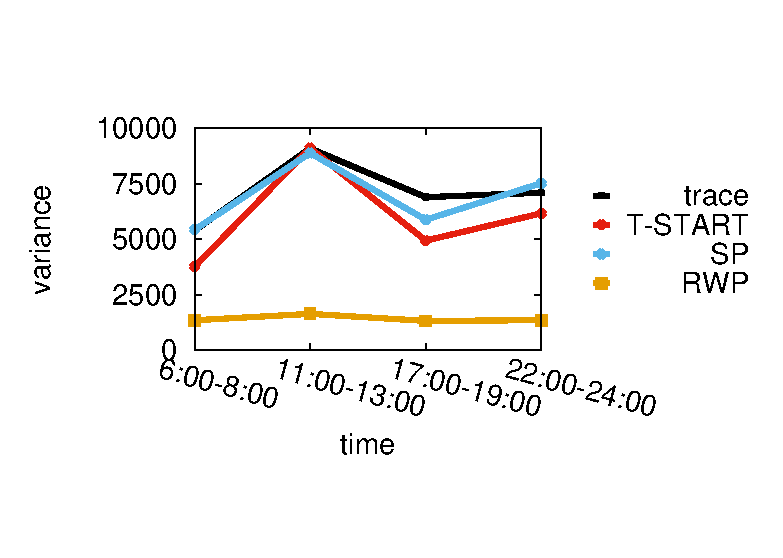
\includegraphics[width=0.5\textwidth]{figures/evalue/indegree/var_out.eps}}
\caption{出入度的均值和方差}\label{figure_avg}
\end{figure}


RWP由于不具有地理特性,其出入度分布较为均匀,如图\ref{figure_indegree_rwp}. 我们集中比较了实际轨迹和本文的出租车移动模型以及SP移动模型。
如图\ref{figure_indegree_dis}所示,图~\ref{figure_indegree_dis}.(a)为实际轨迹在四个事件段上的入度分布图,图\ref{figure_indegree_dis}.(b)为T-START的入度节点分布,图\ref{figure_indegree_dis}.(c)为SP的节点入度分布。由于后两者都是基于地图的移动模型,可以明显的从节点分布的峰值看出其主要的分布在于北京的主要环路上。实际轨迹的入度较为分布十分清晰的分布在环路上,T-START的峰值较为在四环三环路上较为集中,而SP则较为集中于中部。


From figure \ref{figure_indegree_dis}, the peaks of the real traces are contentrated on the main roads. For the T-START and SP use the Dijkstra algrothrithm, they will choose the shortest way to a destination, ignoring the factors of road condition. Nevertheless, we can find out some differences between T-START and SP. The peaks of indegree gather in the middle, because it chose the destination in a random way, while those of T-START distributes more to the ring roads.
\begin{figure}[h]
\centering
\epsfysize=2in\epsfbox{figures/evalue/indegree/17indegree_rwp.eps} 
\caption{从17:00 到 19:00 RWP的入度分布图}\label{figure_indegree_rwp}
\end{figure}
\begin{figure}[!h]
\centering
\begin{tabular}
[c]{ccc}
\epsfysize=1.2in\epsfbox{figures/evalue/indegree/6indegree_trace.eps} &
\epsfysize=1.2in\epsfbox{figures/evalue/indegree/6indegree_start.eps} &
\epsfysize=1.2in\epsfbox{figures/evalue/indegree/6indegree_sp.eps} \\
\epsfysize=1.2in\epsfbox{figures/evalue/indegree/11indegree_trace.eps} &
\epsfysize=1.2in\epsfbox{figures/evalue/indegree/11indegree_start.eps} &
\epsfysize=1.2in\epsfbox{figures/evalue/indegree/11indegree_sp.eps} \\
\epsfysize=1.2in\epsfbox{figures/evalue/indegree/17indegree_trace.eps} &
\epsfysize=1.2in\epsfbox{figures/evalue/indegree/17indegree_start.eps} &
\epsfysize=1.2in\epsfbox{figures/evalue/indegree/17indegree_sp.eps} \\
\epsfysize=1.2in\epsfbox{figures/evalue/indegree/22indegree_trace.eps} &
\epsfysize=1.2in\epsfbox{figures/evalue/indegree/22indegree_start.eps} &
\epsfysize=1.2in\epsfbox{figures/evalue/indegree/22indegree_sp.eps} \\
(a) Traces of Nov.8th & (b) T-START & (c) SP \\
\end{tabular}
\caption{实际轨迹, T-START和SP的入度分布图}\label{figure_indegree_dis}
\end{figure}


为了量化节点出入度的指标,我们引入的相对误差。相对误差的计算公式如公式\ref{equation_relative_err}. 其中分子为每个网格中的出入次数相对于样本的绝对值之和,而分子为样本的网格中出入次数的和。
\begin{equation}
\label{equation_relative_err}
    \delta = \frac{\sum \Delta x}{\sum x_{real}} 
\end{equation}

为了更有效的说明对比的有效性,我们没有讲11月8日的实际轨迹作为对照样本,而是选取了前7天的对应时间段,每个网格的均值,为了说明这个对照具有一致性,排除特殊性的影响,我们分别用前7天的数据对比平均的网格出入度,计算其相对误差,计算结果如表~\ref{table_relative_err_avg}. 表中可以看出,每天的出入度相对于样本的平均值的相对误差不超过$20\%$, 且相对误差较为稳定,均处于一个较低水平,在$9\%-18\%$之间.
由此可知,前7天相对误差的均值可以作为相对误差计算的对照对象。
\begin{table}[!t]
\centering
\caption{每天的出入度对于平均值的相对误差}\label{table_relative_err_avg}
\begin{tabular}[c]{c|c|c|c|c|c|c|c}
\multicolumn{8}{c}{(a) in-degree}\\
\hline
item& 1th&2th&3th&4th&5th&6th&7th\\
\hline
6:00-8:00&
0.1139& 
0.1485&
0.1732&
0.1372&
0.1500&
0.2489&
0.1507\\
11:00-13:00&
0.1056&
0.0953&
0.1509&
0.0994&
0.1714&
0.1294&
0.1011\\
17:00-19:00&
0.1537&
0.1728&
0.1491&
0.1888&
0.1338&
0.1303&
0.1407\\
22:00-24:00&
0.1360&
0.1054&
0.1637&
0.1183&
0.1467&
0.1470&
0.1076\\
\hline
\end{tabular}
\begin{tabular}[c]{c|c|c|c|c|c|c|c}
\multicolumn{8}{c}{(b) out-degree}\\
\hline
item& 1th&2th&3th&4th&5th&6th&7th\\
\hline
6:00-8:00&
0.1132&
0.1481&
0.1726&
0.1374&
0.1499&
0.2478&
0.1507\\
11:00-13:00&
0.1057&
0.0953&
0.1509&
0.0998&
0.1719&
0.1296&
0.1012\\
17:00-19:00&
0.1534&
0.1725&
0.1488&
0.1890&
0.1336&
0.1298&
0.1412\\
22:00-24:00&
0.1358&
0.1057&
0.1636&
0.1184&
0.1468&
0.1469&
0.1075\\
\hline
\end{tabular}
\end{table}

因此,我们计算出11月8日数据,T-START, SP和RWP相对于前7天出入度平均值的相对误差,如图\ref{figure_relative_err}. 11月8日轨迹的出入度在不同时间段均处于一个较低水平,约为$10.5\%-12.8\%$范围内. T-START在各个时间段的相对误差均要明显优于SP和RWP,相对误差处于$46.9\%到49.2\%$范围内。而SP的相对误差在$65.3\%-69.2\%$.而RWP的相对误差超过$80\%$. T-START相对于SP的相对误差减少了$15\%-20\%$.具体相对误差可见附录2.

\begin{figure}[ht]
\centering
\subfigure[relative error of in-degree]{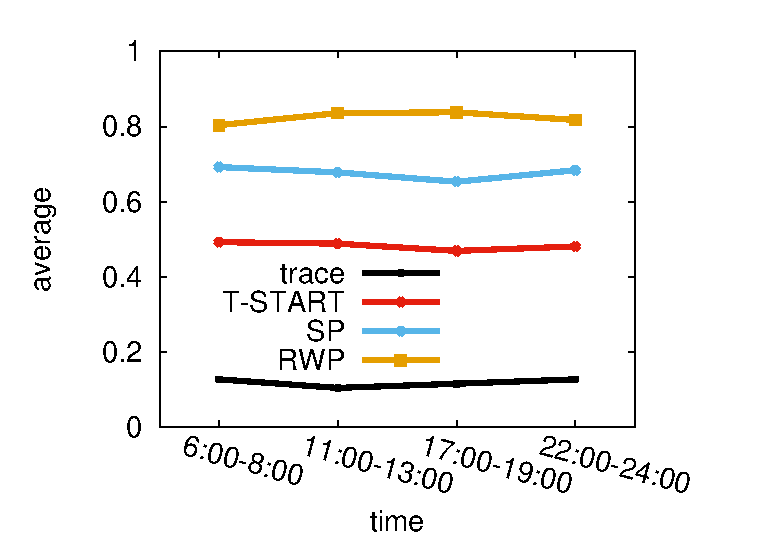
\includegraphics[width=0.45\textwidth]{figures/evalue/indegree/err_in.eps}}
\subfigure[relative error of out-degree]{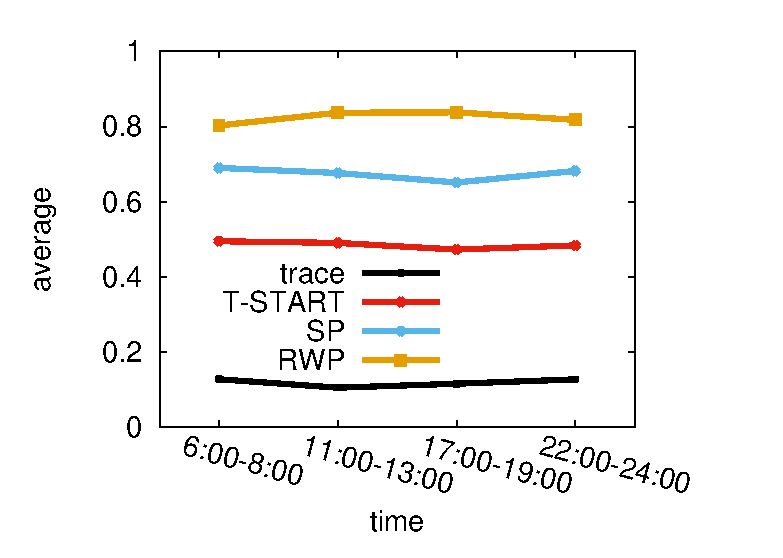
\includegraphics[width=0.45\textwidth]{figures/evalue/indegree/err_out.eps}}
\caption{对前7天的出入度均值矩阵对比的相对误差}\label{figure_relative_err}
\end{figure}

综上所述,T-START从直观角度,节点分布较为分散与实际轨迹比较接近,而SP则比较集中于中心部分,RWP的出入度分布在整个区域内比较集中。通过量化相对于均值的出入度可以看出,每天的出入度相对于网格均值的出入度的相对误差均保持在$9\%-20\%$的较低水平上,11月8日相对于前7天的均值夜较小,因此可以将前7天的出入度的均值矩阵作为对照。实验结果表明T-START具有与均值矩阵较小的相对误差,相对于SP移动模型相对误差减小$15\%-20\%$
\section{接触验证}
\section{本章小结}